\documentclass{standalone}
\usepackage{preset}
\begin{document}
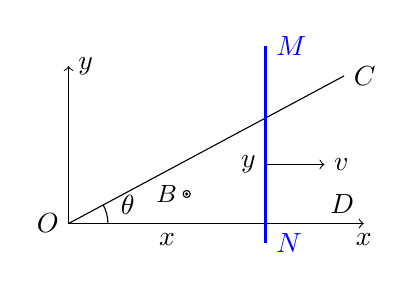
\begin{tikzpicture}[x=25mm,y=25mm]
	\draw[<->](0,.8)node[right]{$y$}--(0,0)--(1.5,0)node[below]{$x$}node[above left]{$D$};
	\draw(0,0)node[left]{$O$}--(1.4,.75)node[right]{$C$};
	\draw[very thick,blue](1,-.1)node[right]{$N$}--(1,.9)node[right]{$M$};
	\draw(.5,0)node[below]{$x$};
	\draw[->](1,.3)node[left]{$y$}--+(.3,0)node[right]{$v$};
	\draw(.2,0)arc(0:28.5:.2)node[right=1mm]{$\theta$};
	\draw[fill=black](.6,.15)circle(.005);
	\draw(.6,.15)circle(.018)node[left]{\small$B$};
\end{tikzpicture}
\end{document}
